\section{Prior Work : Neural Tangent Kernel and Dual View}\label{sec:prelim}
In this section, we will look at \emph{neural tangent kernel} (NTK) theory which gives a kernel interpretation of infinite width DNNs. The open question in the NTK theory is to explain why finite width DNNs outperform the infinite width DNNs. We then look at the dual view, which separately encodes the gates and the weights to: (i) simplify the NTK into a \emph{neural path kernel} which is solely based on the input and the gates and (ii) show that learning in the gates explains why finite width DNNs are better than infinite width DNNs.

\subsection{Infinite Width DNN  = Kernel Method With Neural Tangent Kernel}\label{sec:ntk}
Recent works \citep{ntk,arora2019exact,cao2019generalization} have connected the training and generalisation of DNNs to kernel methods. An important kernel associated with a DNN is its \emph{neural tangent kernel} (NTK), which, for a pair of input examples $x,x'\in\R^{\din}$, and network weights $\Theta\in\R^{\dnet}$, is given by:
\begin{align*}
 \text{NTK}(x,x')\quad = \quad \ip{\nabla_{\Theta}\hat{y}(x), \nabla_{\Theta}\hat{y}(x')}, \quad\text{where}
\end{align*}
$\hat{y}_\Theta(\cdot)\in\R$ is the DNN output. It was shown that, as the width of the DNN goes to infinity, the NTK matrix converges to a limiting deterministic matrix $\text{NTK}_{\infty}$, and training an infinitely wide DNN is equivalent to a kernel method with $\text{NTK}_{\infty}$. \cite{arora2019exact} compared the performance of convolutional neural network with global average pooling (CNN-GAP) and its infinite width Convolutional NTK (CNTK-GAP) on CIFAR-10 and observed the data in \Cref{tb:cntk-cnn}.   Based on the fact that best finite width CNN-GAP ($83.75\%$) performed better than best CNTK-GAP ($77.43\%$) by about $6\%$ they concluded that the infinite width NTK does not explain fully the success of DNNs, and left the characterisation of this performance gap as an interesting \textbf{open question}. 

%\textbf{Open Question 2:} NTK matrix is a fixed matrix and hence there is no feature learning which is at odds with the fact that the success of deep learning is due to feature learning.
\textbf{Remark:} For a proper comparison between the  CNN-GAP and CNTK-GAP, \cite{arora2019exact} avoided tricks such as data augmentation, batch normalisation, dropout and weight decay.
\begin{table}
\begin{tabularx}{\columnwidth}{c *{5}{Y}}
\toprule 
Depth & 3 & 4 & 6&11 &21\\
CNN-GAP &63.81\% &80.93\% & \textbf{83.75}\% & 82.92\% & 83.30\%\\
CNTK-GAP &70.41\% &75.93\% & 76.73\% & \textbf{77.43}\% & 77.08\%\\
\bottomrule
\end{tabularx}
\caption{Data from Table 1 in \citep{arora2019exact}.}
\label{tb:cntk-cnn}
\end{table}


%While these recent results allows us to look at DNNs from the lens of kernels, there are some important issues: (i) \textbf{feature learning:} $\text{NTK}_{\infty}$ being a deterministic matrix does not capture feature learning whereas the success of DNNs is due to feature learning, (ii) \textbf{finite vs infinite width:} finite width convolutional neural network outperforms its corresponding $\text{NTK}_{\infty}$ and (iii)  \textbf{non-interprability:} the NTK is the inner product of gradients and has no physical interpretation. As a result, NTK theory does not fully explain the success of DNNs.

\subsection{Dual View For DNNs with ReLUs: Characterising the role of gates}
We start with describing the encoding of gates, weights, followed by a description of deep gated network setup which separates the gates from the weights, and then we present theoretical results on learning the weights with fixed gates and the experimental results on learning in the gates.
\begin{comment}
\begin{figure}[t]
\resizebox{.95\columnwidth}{!}{
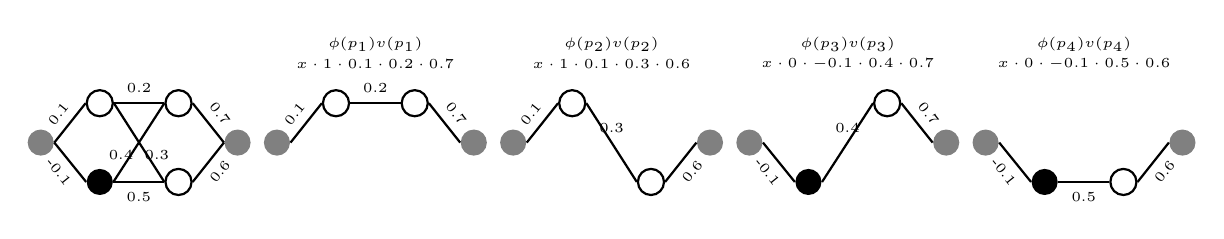
\begin{tikzpicture}
%Top Left
\node[draw,fill=white,circle,thick,
] (tl) at (-0.5,2){};

%Top Right
\node[draw,fill=white,circle,thick,
] (tr) at (0.5,2){};

%Bottom Left
\node[fill=black,circle,
] (bl) at (-0.5,1){};

%Bottom Right
\node[draw,fill=white,circle,thick,
] (br) at (0.5,1){};


%Input
\node[fill=gray,circle,
] (input) at (-1.25,1.5){};


%Output
\node[fill=gray,circle,
] (output) at (1.25,1.5){};

\draw[-, thick] (input.east) -- (tl.west) node [midway, above, sloped] (t1) {\tiny{0.1}};
\draw[-, thick] (input.east) -- (bl.west) node [midway, below, sloped] (t2) {\tiny{-0.1}};
\draw[-, thick] (tl.east) -- (tr.west) node [midway, above, sloped] (t1) {\tiny{0.2}};
\draw[-, thick] (bl.east) -- (br.west) node [midway, below, sloped] (t1) {\tiny{0.5}};
\draw[-, thick] (tl.east) -- (br.west) node [pos=0.85, above] (t1) {\tiny{0.3}};
\draw[-, thick] (bl.east) -- (tr.west) node [pos=0.15, above] (t1) {\tiny{0.4}};
\draw[-, thick] (tr.east) -- (output.west) node [midway, above, sloped] (t1) {\tiny{0.7}};
\draw[-, thick] (br.east) -- (output.west) node [midway, below, sloped] (t1) {\tiny{0.6}};




%%%%%%%%%%%%%%%%%Path 1%%%%%%%%%%%%%%
%Input
\node[fill=gray,circle,
] (p1input) at (1.75,1.5){};


%Output
\node[fill=gray,circle,
] (p1output) at (4.25,1.5){};



%Top Left
\node[draw,fill=white,circle,thick,
] (p1tl) at (2.5,2){};

%Top Right
\node[draw,fill=white,circle,thick,
] (p1tr) at (3.5,2){};




\draw[-, thick] (p1input.east) -- (p1tl.west) node [midway, above, sloped] (t1) {\tiny{0.1}};
\draw[-, thick] (p1tl.east) -- (p1tr.west) node [midway, above, sloped] (t1) {\tiny{0.2}};
\draw[-, thick] (p1tr.east) -- (p1output.west) node [midway, above, sloped] (t1) {\tiny{0.7}};



%%%%%%%%%%%%%%%%%Path 2%%%%%%%%%%%%%%

%Input
\node[fill=gray,circle,
] (p2input) at (4.75,1.5){};


%Output
\node[fill=gray,circle,
] (p2output) at (7.25,1.5){};

%Top Left
\node[draw,fill=white,circle,thick,
] (p2tl) at (5.5,2){};

%Bottom Right
\node[draw,fill=white,circle,thick,
] (p2br) at (6.5,1){};

\draw[-, thick] (p2input.east) -- (p2tl.west) node [midway, above, sloped] (t1) {\tiny{0.1}};
\draw[-, thick] (p2tl.east) -- (p2br.west) node [pos=0.5, above] (t1) {\tiny{0.3}};
\draw[-, thick] (p2br.east) -- (p2output.west) node [midway, below, sloped] (t1) {\tiny{0.6}};



%%%%%%%%%%%%%%%%%Path 3%%%%%%%%%%%%%%

%Input
\node[fill=gray,circle,
] (p3input) at (7.75,1.5){};


%Output
\node[fill=gray,circle,
] (p3output) at (10.25,1.5){};


%Top Right
\node[draw,fill=white,circle,thick,
] (p3tr) at (9.5,2){};

%Bottom Left
\node[fill=black,circle,
] (p3bl) at (8.5,1){};



\draw[-, thick] (p3input.east) -- (p3bl.west) node [midway, below, sloped] (t2) {\tiny{-0.1}};
\draw[-, thick] (p3bl.east) -- (p3tr.west) node [pos=0.5, above] (t1) {\tiny{0.4}};
\draw[-, thick] (p3tr.east) -- (p3output.west) node [midway, above, sloped] (t1) {\tiny{0.7}};


%%%%%%%%%%%%%%%%%Path 4%%%%%%%%%%%%%%

%Input
\node[fill=gray,circle,
] (p4input) at (10.75,1.5){};


%Output
\node[fill=gray,circle,
] (p4output) at (13.25,1.5){};

%Bottom Left
\node[fill=black,circle,
] (p4bl) at (11.5,1){};

%Bottom Right
\node[draw,fill=white,circle,thick,
] (p4br) at (12.5,1){};

\draw[-, thick] (p4input.east) -- (p4bl.west) node [midway, below, sloped] (t2) {\tiny{-0.1}};
\draw[-, thick] (p4bl.east) -- (p4br.west) node [midway, below, sloped] (t1) {\tiny{0.5}};
\draw[-, thick] (p4br.east) -- (p4output.west) node [midway, below, sloped] (t1) {\tiny{0.6}};
%%%%%%%%%%%%%%%%%%%%%%%%%%%%%%

\node[] () at (3,2.75){\tiny{$\phi(p_1)v(p_1)$}};
\node[] () at (3,2.5){\tiny{$x\cdot 1\cdot 0.1 \cdot 0.2 \cdot 0.7$}};

\node[] () at (6,2.75){\tiny{$\phi(p_2)v(p_2)$}};
\node[] () at (6,2.5){\tiny{$x\cdot 1\cdot 0.1 \cdot 0.3 \cdot 0.6$}};

\node[] () at (9,2.75){\tiny{$\phi(p_3)v(p_3)$}};
\node[] () at (9,2.5){\tiny{$x\cdot 0\cdot -0.1 \cdot 0.4 \cdot 0.7$}};

\node[] () at (12,2.75){\tiny{$\phi(p_4)v(p_4)$}};
\node[] () at (12,2.5){\tiny{$x\cdot 0\cdot -0.1 \cdot 0.5 \cdot 0.6$}};




\end{tikzpicture}


}
\caption{\small{Illustration of the dual `path-by-path' view of computations in a toy network with an input node, $2$ layer and $2$ hidden units in each layer and an output node. . Let us say for this particular input $x$, the bottom ReLU/gate in the first layer is `off/inactive' and rest of the ReLUs are `on/active'. In this case , paths $p_1$ and $p_2$ are active and paths $p_3$ and $p_4$ are inactive. }}
\label{fig:paths}
\end{figure}
\end{comment}
\subsubsection{Neural Path Features, Neural Path Value and Neural Path Kernel}
Consider a fully connected DNN with `$d$' layers and `$w$' hidden units in each layer. Let the DNN accept input $x\in \R^{\din}$ and produce an output $\hat{y}_{\Theta}(x)\in\R$. %Let a path be defined to be one that starts from an input node, passes through a weight and a hidden unit in each layer and ends at the output node. There are $\Pfc= \din w^{(d-1)}$ paths, let them be enumerable as $p=1,\ldots, \Pfc$. Let the index of the hidden unit in layer $l$ through which a path $p$ passes be denoted by $\I_l(p), l=0,1,\ldots,d$, where $l=0$ means the input layer. Let $\Theta\in\R^{\dnet}$ be the weights of network, with $\Theta(l,i,j)$ denoting the weight connecting the $i^{th}$ unit in layer $l$ and the $j^{th}$ unit in layer $l-1$. Let $G_l(x,I_l(p))$ denote the gate in the $l^{th}$ layer in path $p$. The neural path feature encoding the input and gates, and the neural path value encoding the weights is defined as below.
\begin{definition}\label{def:npf-npv}
A path starts from an input node, passes through a weight and a hidden unit in each layer and ends at the output node. We define the following quantities for a path $p$:
\begin{comment}
\begin{tabular}{lccl}
 Activity&:& $A_{\Theta}(x,p)$&=$\quad\Pi_{l=1}^{d-1} G_l\left(x,\I_l(p)\right)$.\\
Value&:& $v_{\Theta}(p)$&=$\quad\Pi_{l=1}^d\Theta\left(l,\I_{l-1}(p),\I_{l}(p)\right)$.\\
Feature&:&   $\phi_{\Theta}(x,p)$&=$\quad x\left(\I_0(p)\right)A_{\Theta}(x,p)$.
\end{tabular}
\end{comment}
\emph{
\begin{tabular}{lcl}
 Activity&:& $A_{\Theta}(x,p)$ is the product of the `$d-1$' gates in the path. \\
Value&:& $v_{\Theta}(p)$ is the product of the `$d$' weights in the path.\\
Feature&:&   $\phi_{\Theta}(x,p)$ is the product of the signal at the input node of the path and $A_{\Theta}(x,p)$.\\
\end{tabular}
}
The \emph{neural path feature} (NPF) given by $\phi_{\Theta}(x)=\left(\phi_{\Theta}(x,p),p=1,\ldots, \Pfc\right),\in\R^{\Pfc}$ and the \emph{neural path value} (NPV) given by $v_{\Theta}=\left(v_{\Theta}(p),p=1,\ldots,\Pfc\right),\in\R^{\Pfc}$.
\end{definition}
Note that the neural path features are completely dictated by the gates, and i.e., if any gate in a path $p$ is not active for a given input $x\in\R^{\din}$, then $\phi(x,p)=0$.
\begin{proposition}\label{prop:npf-npv}
The output of the DNN is then the inner product of the NPF and NPV: 
\begin{align}\label{eq:inner}
\hat{y}_{\Theta}(x)=\ip{\phi_{\Theta}(x),v_{\Theta}}=\sum_{p\in[P]}  \phi_{\Theta}(x,p) v_{\Theta}(p)
\end{align}
\end{proposition}
\textbf{Subnetwork Interpretation of DNNs with ReLUs.} A path is active only if all the gates in the path are active. This gives a subnetwork interpretation, i.e., for a given input $x\in\R^{\din}$ only a subset gates and consequently only a subset of paths are active (i.e., paths for which $A(x,p)=1$), and the input to output computation can be seen to be produced by this subnetwork. The following matrix captures the correlation of the active subnetworks for a given pair of inputs $x,x'\in\R^{\din}$.
\begin{definition}[Overlap of active sub-networks]\label{def:overlap} 
The total number of `active' paths for both $x$ and $x'$ that pass through input node $i$ is defined to be:

{\centering{$\textbf{overlap}_{\Theta}(i,x,x') \eqdef {\left|\{p \colon  \I_0(p)=i \,, A_{\Theta}(x,p)= A_{\Theta}(x',p)=1\} \right|}$}\par}
\end{definition}
\begin{lemma}[Neural Path Kernel (NPK)]\label{lm:npk}
Let $D\in\R^{\din}$ be a vector of non-negative entries  and for $u,u'\in\R^{\din}$ , let $\ip{u,u'}_{D}=\sum_{i=1}^{\din}D(i)u(i)u'(i)$. Then the neural path kernel (NPK) is given by: 
\begin{align*} 
\text{NPK}_{\Theta}(x,x')\eqdef \ip{\phi_{\Theta}(x),\phi_{\Theta}(x')}= \ip{x,x'}_{\textbf{overlap}_{\Theta}(\cdot,x,x')} 
\end{align*}
\end{lemma}



%Each path transmits the signal equal to the neural path feature $\phi(x,p)$ which on its way to the output is scaled by the neural path value $v(p)$  which is equal the product of the weights in the path. 

\begin{comment}
\begin{figure}[t]
\centering
\resizebox{0.9\columnwidth}{!}{
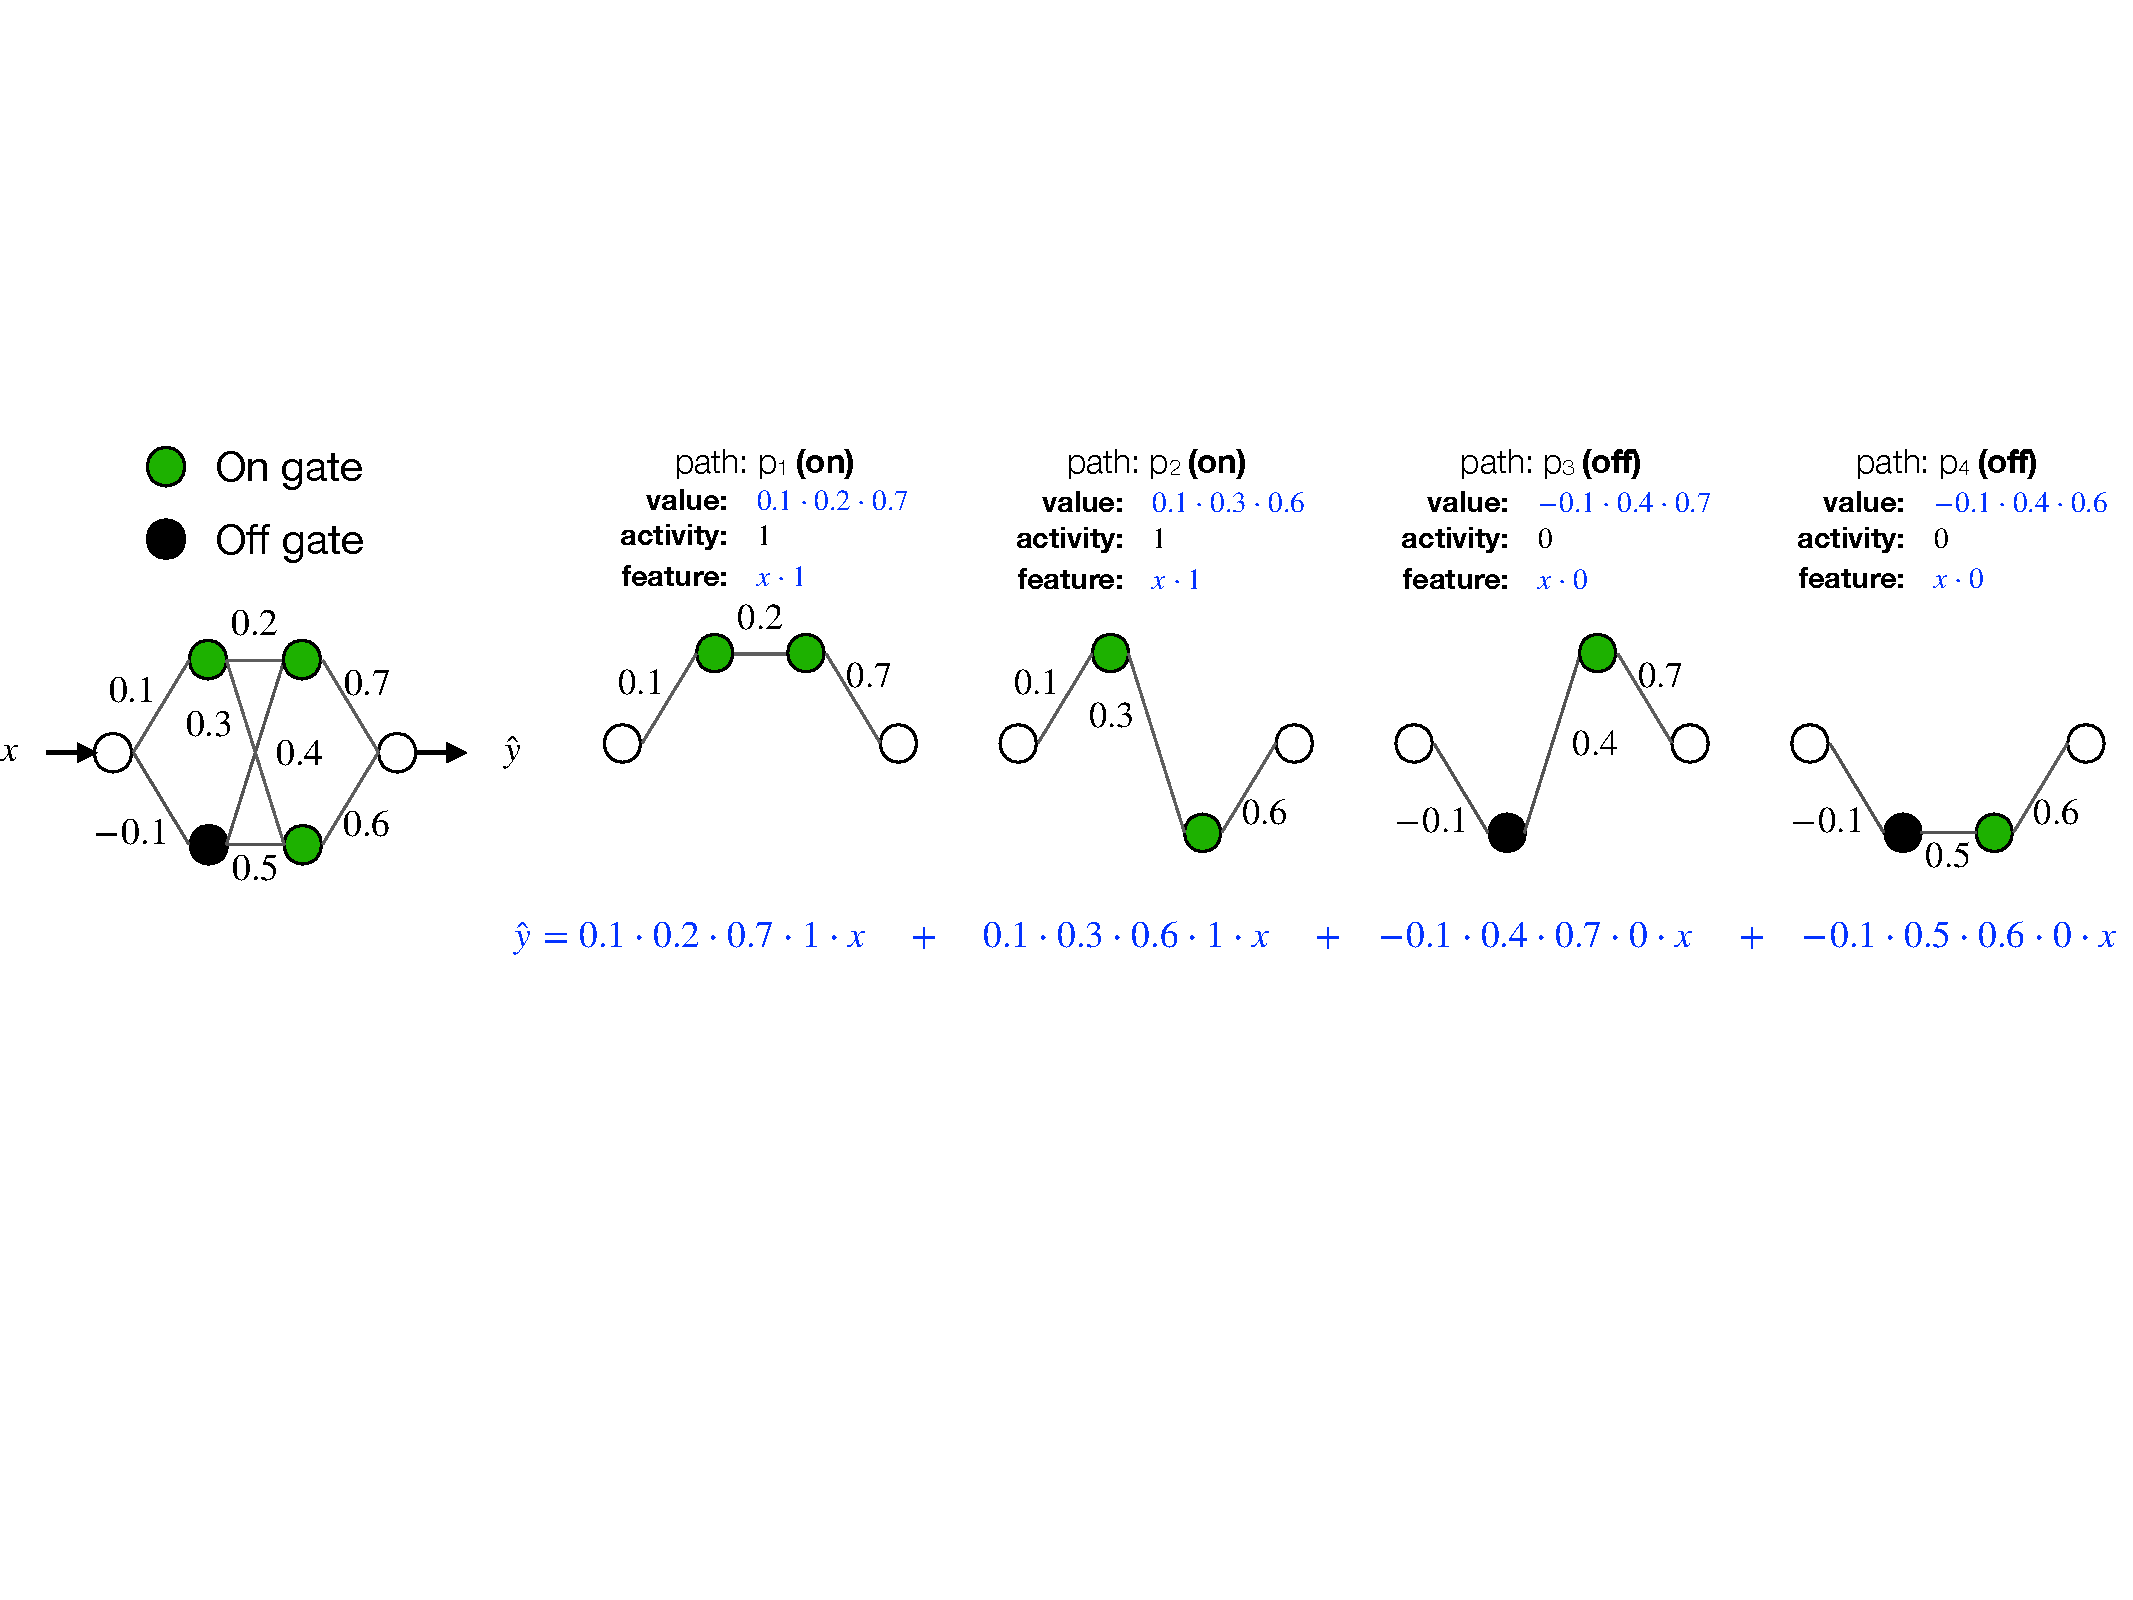
\includegraphics[scale=0.5]{figs/paths.pdf}
}
\caption{Illustration of \Cref{def:npf-npv} and \Cref{prop:npf-npv} in a  toy network with $2$ layers, $2$ gates per layer and $4$ paths. Paths $p_1$ and $p_2$ are `on' and paths $p_3$ and $p_4$ are `off'. The value, activity and feature of the individual paths are shown. $\hat{y}$ is the summation of the individual path contributions.}
\label{fig:paths}
\end{figure}

\begin{figure}
\centering
\begin{minipage}{0.8\columnwidth}
\begin{minipage}{0.49\columnwidth}
\resizebox{0.85\columnwidth}{!}{
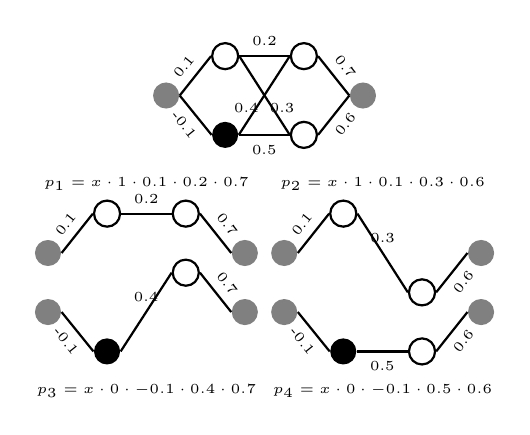
\begin{tikzpicture}
%Top Left
\node[draw,fill=white,circle,thick,
] (tl) at (-0.5,1.75){};

%Top Right
\node[draw,fill=white,circle,thick,
] (tr) at (0.5,1.75){};

%Bottom Left
\node[fill=black,circle,
] (bl) at (-0.5,0.75){};

%Bottom Right
\node[draw,fill=white,circle,thick,
] (br) at (0.5,0.75){};


%Input
\node[fill=gray,circle,
] (input) at (-1.25,1.25){};


%Output
\node[fill=gray,circle,
] (output) at (1.25,1.25){};

\draw[-, thick] (input.east) -- (tl.west) node [midway, above, sloped] (t1) {\tiny{0.1}};
\draw[-, thick] (input.east) -- (bl.west) node [midway, below, sloped] (t2) {\tiny{-0.1}};
\draw[-, thick] (tl.east) -- (tr.west) node [midway, above, sloped] (t1) {\tiny{0.2}};
\draw[-, thick] (bl.east) -- (br.west) node [midway, below, sloped] (t1) {\tiny{0.5}};
\draw[-, thick] (tl.east) -- (br.west) node [pos=0.85, above] (t1) {\tiny{0.3}};
\draw[-, thick] (bl.east) -- (tr.west) node [pos=0.15, above] (t1) {\tiny{0.4}};
\draw[-, thick] (tr.east) -- (output.west) node [midway, above, sloped] (t1) {\tiny{0.7}};
\draw[-, thick] (br.east) -- (output.west) node [midway, below, sloped] (t1) {\tiny{0.6}};




%%%%%%%%%%%%%%%%%Path 1%%%%%%%%%%%%%%
%Input
\node[fill=gray,circle,
] (p1input) at (-2.75,-0.750){};


%Output
\node[fill=gray,circle,
] (p1output) at (-0.25,-0.750){};



%Top Left
\node[draw,fill=white,circle,thick,
] (p1tl) at (-2.0,-0.25){};

%Top Right
\node[draw,fill=white,circle,thick,
] (p1tr) at (-1.0,-0.25){};




\draw[-, thick] (p1input.east) -- (p1tl.west) node [midway, above, sloped] (t1) {\tiny{0.1}};
\draw[-, thick] (p1tl.east) -- (p1tr.west) node [midway, above, sloped] (t1) {\tiny{0.2}};
\draw[-, thick] (p1tr.east) -- (p1output.west) node [midway, above, sloped] (t1) {\tiny{0.7}};



%%%%%%%%%%%%%%%%%Path 2%%%%%%%%%%%%%%

%Input
\node[fill=gray,circle,
] (p2input) at (0.25,-0.750){};


%Output
\node[fill=gray,circle,
] (p2output) at (2.75,-0.750){};

%Top Left
\node[draw,fill=white,circle,thick,
] (p2tl) at (1,-0.25){};

%Bottom Right
\node[draw,fill=white,circle,thick,
] (p2br) at (2,-1.25){};

\draw[-, thick] (p2input.east) -- (p2tl.west) node [midway, above, sloped] (t1) {\tiny{0.1}};
\draw[-, thick] (p2tl.east) -- (p2br.west) node [pos=0.5, above] (t1) {\tiny{0.3}};
\draw[-, thick] (p2br.east) -- (p2output.west) node [midway, below, sloped] (t1) {\tiny{0.6}};



%%%%%%%%%%%%%%%%%Path 3%%%%%%%%%%%%%%

%Input
\node[fill=gray,circle,
] (p3input) at (-2.75,-1.5){};


%Output
\node[fill=gray,circle,
] (p3output) at (-0.25,-1.5){};


%Top Right
\node[draw,fill=white,circle,thick,
] (p3tr) at (-1,-1){};

%Bottom Left
\node[fill=black,circle,
] (p3bl) at (-2,-2){};



\draw[-, thick] (p3input.east) -- (p3bl.west) node [midway, below, sloped] (t2) {\tiny{-0.1}};
\draw[-, thick] (p3bl.east) -- (p3tr.west) node [pos=0.5, above] (t1) {\tiny{0.4}};
\draw[-, thick] (p3tr.east) -- (p3output.west) node [midway, above, sloped] (t1) {\tiny{0.7}};


%%%%%%%%%%%%%%%%%Path 4%%%%%%%%%%%%%%

%Input
\node[fill=gray,circle,
] (p4input) at (0.25,-1.50){};


%Output
\node[fill=gray,circle,
] (p4output) at (2.75,-1.50){};

%Bottom Left
\node[fill=black,circle,
] (p4bl) at (1,-2){};

%Bottom Right
\node[draw,fill=white,circle,thick,
] (p4br) at (2,-2){};

\draw[-, thick] (p4input.east) -- (p4bl.west) node [midway, below, sloped] (t2) {\tiny{-0.1}};
\draw[-, thick] (p4bl.east) -- (p4br.west) node [midway, below, sloped] (t1) {\tiny{0.5}};
\draw[-, thick] (p4br.east) -- (p4output.west) node [midway, below, sloped] (t1) {\tiny{0.6}};


%%%%%%%%%%%%%%%%%%%%%%%%%%%%%%%%%%%%%%%%%%%%

\node[] () at (-1.5,0.125){\tiny{$p_1=x\cdot 1\cdot 0.1 \cdot 0.2 \cdot 0.7$}};

\node[] () at (1.5,0.125){\tiny{$p_2=x\cdot 1\cdot 0.1 \cdot 0.3 \cdot 0.6$}};

\node[] () at (-1.5,-2.5){\tiny{$p_3=x\cdot 0\cdot -0.1 \cdot 0.4 \cdot 0.7$}};

\node[] () at (1.5,-2.5){\tiny{$p_4=x\cdot 0\cdot -0.1 \cdot 0.5 \cdot 0.6$}};




\end{tikzpicture}


}
\end{minipage}
\begin{minipage}{0.49\columnwidth}
\resizebox{0.99\columnwidth}{!}{
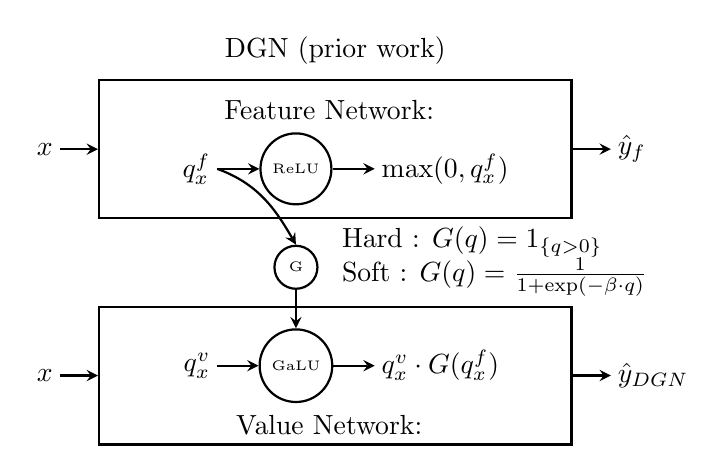
\begin{tikzpicture}

\node []  (fntext)at (3.5,1.5) {DGN (prior work)};
%Feature Network
\node [draw,
	minimum width=6cm,
	minimum height=1.75cm,
	thick
]  (fnbox)at (3.5,0.25) {};
\node []  (fntext)at (3.5,0.75) {Feature Network: $\Tf$};


%Feature Network Input
\node (fin) [left of=fnbox,node distance=3.5cm, coordinate] {};
\node[left=-1pt] at (fin.west){$x$};
\draw[-stealth, thick] (fin.center) -- (fnbox.west);

%Feature Network Output
\node (fout) [right of=fnbox,node distance=3.5cm, coordinate] {};
\node[right=-1pt] at (fout.west){$\hat{y}_{\text{f}}$};
\draw[-stealth, thick]  (fnbox.east)--(fout.center);


%ReLU Circle
\node[draw,
	circle,
	minimum size=0.75cm,thick,
] (relu) at (3,0){\tiny{ReLU}};
%ReLU Input
\node (b) [left of=relu,node distance=1cm, coordinate] {};

\node[left=-1pt] at (b.center){$q^\text{f}_x$};
\draw[-stealth, thick] (b.east) -- (relu.west);


%ReLU Output
\node (c) [right of=relu,node distance=1cm, coordinate] {};
\node[right=-1pt] at (c.center){$\max(0,q^\text{f}_x)$};
\draw[-stealth, thick] (relu.east) -- (c.west);
	

%Gating Circle
\node[draw,
	circle,
	minimum size=0.0625cm,thick,
] (gating) at (3,-1.25){\tiny{G}};
%\node[right=6pt] at (gating.north){Hard : $G(q)=\mathbbm{1}_{\{q>0\}} $};
%\node[below right=6pt] at (gating.north){Soft : $G(q)=\frac{1}{1+\exp(-\beta\cdot q)}$};

\node[right=6pt] at (3.25,-0.925){Hard : $G(q)=\mathbbm{1}_{\{q>0\}} $};
\node[right=6pt] at (3.25,-1.375){Soft : $G(q)=\frac{1}{1+\exp(-\beta\cdot q)}$};


%Value Network

\node [draw,
	minimum width=6cm,
	minimum height=1.75cm,
	thick
]  (vnbox)at (3.5,-2.625) {};

\node []  (vntext)at (3.5,-3.25) {Value Network: $\Tv$};

%Value Network Input
\node (vin) [left of=vnbox,node distance=3.5cm, coordinate] {};
\node[left=-1pt] at (vin.west){$x$};
\draw[-stealth, thick] (vin.center) -- (vnbox.west);

%Feature Network Input
\node (vout) [right of=vnbox,node distance=3.5cm, coordinate] {};
\node[right=-1pt] at (vout.west){$\hat{y}_{\text{DGN}}$};
\draw[-stealth, thick]  (vnbox.east)--(vout.center);



%GaLU Circle
\node[draw,
	circle,
	minimum size=0.75cm,thick,
] (galu) at (3,-2.5){\tiny{GaLU}};

\draw [-stealth,thick]   (b) to[out=-20,in=120] (gating.north);
\draw [-stealth,thick]   (gating.south) -- (galu.north);


%GaLU Input
\node (d) [left of=galu,node distance=1cm, coordinate] {};
\node[left=-1pt] at (d.center){$q^\text{v}_x$};
\draw[-stealth, thick] (d.east) -- (galu.west);
%GaLU Output
\node (e) [right of=galu,node distance=1cm, coordinate] {};
\node[right=-1pt] at (e.center){$q^\text{v}_x\cdot G(q^\text{f}_x)$};
\draw[-stealth, thick] (galu.east) -- (e.west);
	
\end{tikzpicture}


}
\end{minipage}
\end{minipage}
\caption{DGN}
\label{fig:dgn}
\end{figure}
\end{comment}
%As mentioned in \Cref{sec:intro}, a deep gated network(DGN) setup is an alternative way to compute path-by-path, that is, the to compute the inner product of the neural path feature and neural path value. In this section, we first describe DGN in prior work \citep{npk}:  consitituent parts, information flow, purpose and training. We then discuss the two fundamental conceptual issues that make this DGN `black box'. We then present our modified \texttt{DGN-NO-ACT} with an intutitve explanation of how the conceptual issues are overcome and  why it is an entirely interpretatble white box model. These intuitive explanations will be justified in theory and experiments in \Cref{sec:main}.
\subsubsection{Deep Gated Network: Separating Gates and Weights}
\textbf{Deep Gated Network (DGN)} is a setup to separate the gates from the weights. Consider a DNN with ReLUs with weights $\Theta\in\R^{\dnet}$. The DGN \emph{corresponding} to this DNN (see the left diagram in \Cref{fig:dgn}) has two networks of \emph{identical architecture} (to the DNN) namely the `gating network' and the `weight network' with distinct weights $\Tf\in\R^{\dnet}$ and $\Tv\in\R^{\dnet}$ respectively.  
%The main difference between the feature and value networks is in the activations. 
The `gating network' has ReLUs which turn `on/off' based on their pre-activation signals, and the `weight network' has gated linear units (GaLUs) \citep{sss,npk}, which multiply their respective pre-activation inputs by the external gating signals provided by the `gating network'.  Since the gating and weight networks have identical architecture, there is a one-to-one correspondence between the ReLUs and GaLUs in the respective networks.  Gating network realises $\phi_{\Tf}(x)$ by turning `on/off' the corresponding GaLUs in the weight network. The weight network realises $v_{\Tv}$ and computes the output $\hat{y}_{\text{DGN}}(x)=\ip{\phi_{\Tf}(x),v_{\Tv}}$.  The gating network is also called the feature network since it realises the neural path features, and the weight network is also called as the value network since it realises the neural path value. Training of DGN is explained in \Cref{sec:gatelearning}.

%In the DGN, the external gating signal to the GaLU is derived from the pre-activation input of the corresponding ReLU. 

%The feature network computes the pre-activations in a layer-by-layer manner, the pre-activations from the feature network generate the gates, which are then used to switch

\subsubsection{Learning Weights With Fixed Gates = Neural Path Kernel}
During training, a DNN learns both $\phi_{\Theta}(x)$ as well as $v_{\Theta}$ simultaneously, and a finite time characterisation of this learning in finite width DNNs is desirable. However, this is a hard problem. A slightly easier problem is to understand in a DGN, how the weights in the value network are learnt when the gates are fixed in the feature network, i.e., how the relation $\hat{y}_{DGN}(x)=\ip{\phi_{\Tf}(x),v_{\Tv}}$ is learnt by learning $v_{\Tv}$ with fixed $\phi_{\Tf}(x)$. This is a linear model in dual variables, which we call as \textbf{dual linearity}. Note that $\hat{y}_{DGN}(x)=\ip{\phi_{\Tf}(x),v_{\Tv}}$ is still non-linear in the value network weights $\Tv$. However, dual linearity has a kernel interpretation in the \emph{infinite width regime}. \cite{npk} showed that the dual linearity is characterised by the NPK in the infinite width regime. We state the assumption followed by Theorem 5.1 in \citep{npk}.

\begin{assumption}\label{assmp:main}
$\Tv_0\stackrel{\text{i.i.d}}\sim\text{Bernoulli}(\frac12)$ over $\{-{\sigma},+{\sigma}\}$ and statistically independent of $\Tf_0$.
\end{assumption}
%We point out that this statistical decoupling of weights and gates in \Cref{assmp:main} is unrealisable in a DNN with ReLU, however, this assumption can be trivially realised in a DGN. %Further, we are interested only in the `what?' ( and not `how?') question related to the gates in which case this assumptions is not a restriction.

\begin{theorem}[Theorem 5.1 in \citep{npk}]
\label{th:fcprev} Under \Cref{assmp:main} for FC-DGN : 
\begin{align*}
\text{NTK}=(x,x') \stackrel{(a)}\rightarrow &d \cdot \sigma^{2(d-1)} \cdot \text{NPK}(x,x'), \quad\text{as}\,\, w\rightarrow \infty \\
					     & = d \cdot \sigma^{2(d-1)}\cdot\ip{x,x'}\cdot \textbf{overlap}(x,x')
\end{align*}
\end{theorem} 
\textbf{Remark.} In \Cref{th:fcprev}, since the gates are fixed, the NTK is due to the gradient of $\hat{y}_{\text{DGN}}$ with respect to the value network weights. Also, note that in the fully connected case, $\textbf{overlap}(i,x,x')$ is identical for all $i=1,\ldots,\din$, and hence $\ip{x,x'}_{\textbf{overlap}(\cdot,x,x')}$ in \Cref{lm:npk} becomes $\ip{x,x'}\cdot \textbf{overlap}(x,x')$.
\subsubsection{Learning in Gates : Why Finite Width Is Better Than Infinite Width}\label{sec:gatelearning}
While the fixed gates setting is an idealised setting, it helps in comparing \textbf{fixed learnt (FL)}  gates coming from a pre-trained DNN and \textbf{fixed random (FR)} gates coming from randomly initialised DNN, and the infinite width NTK.  \cite{npk} compared the performance of a $4$ layer CNN-GAP with its corresponding `Convolutional DGN-GAP' (CDGN-GAP) on CIFAR-10 and the observed the results in \Cref{tb:cdgn}. Since the fixed random (FR) gates performed poorly ($67.09\%$) than the best CNTK in \citep{arora2019exact} ($77.43\%$) and the fixed learnt (FL) gates performed better ($79.68\%$) than the best CNTK, it was concluded that learning in the gates or neural path feature learning explains the why finite width CNN-GAP outperforms the infinite width CNTK-GAP; this \textbf{explains the open questions} in \Cref{sec:ntk}. It was also shown that if the gates are not fixed but allowed to learn along with the weights the performance is \emph{marginally poor} compared to the DNN. This is shown as the \textbf{learnable gates} in \Cref{fig:dgn,tb:cdgn}. 
\begin{table}
\begin{tabularx}{\columnwidth}{c *{4}{Y}}
\toprule 
CNN-GAP & \multicolumn{3}{c} {CDGN-GAP} \\\cline{2-4}
& Fixed Learnt Gates & Fixed Random Gates & Learnable Gates\\
80.32\% & 79.68\% &67.09\% & 77.12\%\\
\bottomrule
\end{tabularx}
\caption{Data from Table 2 in \citep{npk}.}
\label{tb:cdgn}
\end{table}


%The information in the gates or the performance of the gates is measured by keeping the gates fixed in the feature network and training the weights of the value network. The key result in \citep{npk} was that the learning in the gates (i.e., the neural path features) improves generalisation, and is the reason behind why finite width DNNs outperforms the infinite width NTK. This result was established empirically by comparing the performance of \textbf{fixed learnt (FL)} gates and that of \textbf{fixed random(FR)} gates and the performance of the NTK in \cite{arora2019exact}. The fixed learnt gates are those that come from a pre-trained feature network (pre-trained using $\hat{y}_\text{f}$) and the fixed random gates are those that come from a randomly initialised feature network. For this purpose, \citep{npk} used a `C4GAP' architecture with $4$ convolutional layers, followed by global-average-pooling (GAP) and a fully connected layer with `softmax' activations. On CIFAR-10, it was observed that the fixed random (FR) gates performed poorly ($68.08\%$) than the NTK in \citep{arora2019exact} ($77.43$) and the fixed learnt (FL) gates performed better ($79.68\%$) than the NTK and within $1\%$ to the C4GAP-DNN ($80.32\%$). Based on this observation it was concluded that (i) gates (encoded as neural path features) are learnt, and (ii) the learning in the gates is the reason for finite width DNN outperforming infinite width NTK. It was also shown that the DGN can be trained standalone, i.e., gates in the feature network and the weights in the value network can be learnt starting from randomised initialisation. The standalone DGN performed only \emph{marginally poor} ($77.12\%$) compared to the DNN ($80.32\%$).

%The test accuracy of C4GAP is approximately $80\%$ on CIFAR-10, and is not state of the art.  However, the main aim here was to compare with the corresponding infinite width NTK whose performance was $77.34\%$ \citep{arora2019exact} for which the C4GAP was sufficient. 



%In a DNN with ReLUs, both the gates (encoded in the neural path features) and the weights (encoded in the neural path value) are learnt by the DNN itself. The DGN setup helps to separate out the learning in the gates (which are learnt in the feature network) and  from the learning in the weights (which are learnt in the value network). Using the DGN, the information in the gates can be measured, by keeping the gates fixed and then training the weights alone. This is equivalent to asking `how good are the neural path features?' and answering it by keeping $\phi_{\Tf}(x)$ fixed and training $v_{\Tv}$ to learn the relation $\hat{y}_{\text{DGN}}(x)=\ip{\phi_{\Tf}(x),v_{\Tv}}$. We now briefly main result in \citep{npk} on fixing gates and learning weights.

%{\centering \emph{{What is the analysis for fixing the gates, i.e., $\phi_{\Tf}(x)$ and learning the weights, i.e., $v_{\Tv}$?}}\par}

%\textbf{Analytical Characterisation of Learning Weights Given Gates.} Recent works \citep{ntk,arora2019exact,cao2019generalization} have connected the training and generalisation of DNNs to kernel methods. An important kernel associated with a DNN is its \emph{neural tangent kernel} (NTK), which, for a pair of input examples $x,x'\in\R^{\din}$, and network weights $\Theta\in\R^{\dnet}$, is given by:
%\begin{align*}
% \text{NTK}(x,x')\quad = \quad \ip{\nabla_{\Theta}\hat{y}(x), \nabla_{\Theta}\hat{y}(x')}
% \end{align*}
%It was shown that, as the width of the DNN goes to infinity, the NTK matrix converges to a limiting deterministic matrix $\text{NTK}_{\infty}$, and training an infinitely wide DNN is equivalent to a kernel method with $\text{NTK}_{\infty}$. Theorem 5.1 in \citep{npk} showed that, when the gates are fixed,  at randomised initialisation, the NTK of an  infinitely wide DGN is equal to (but for a constant factor) the neural path kernel (NPK) which is the Gram matrix of the neural path features. 

%\textbf{Remark:} A previously unnoticed property of the NPK was that it is invariant to layer permutations. Theorem 5.1 in \citep{npk} is not presented here, it is restated in \Cref{th:fc} in which the invariance property is made explicit. 

\begin{figure}
\centering
\begin{minipage}{0.8\columnwidth}
\centering
\begin{minipage}{0.45\columnwidth}
\resizebox{1.0\columnwidth}{!}{
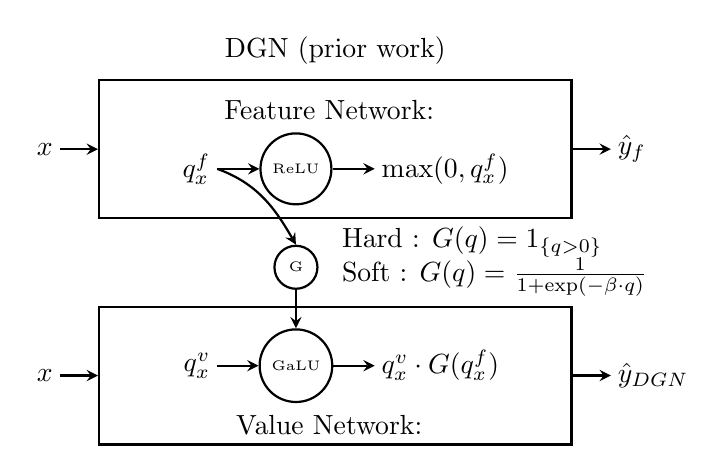
\begin{tikzpicture}

\node []  (fntext)at (3.5,1.5) {DGN (prior work)};
%Feature Network
\node [draw,
	minimum width=6cm,
	minimum height=1.75cm,
	thick
]  (fnbox)at (3.5,0.25) {};
\node []  (fntext)at (3.5,0.75) {Feature Network: $\Tf$};


%Feature Network Input
\node (fin) [left of=fnbox,node distance=3.5cm, coordinate] {};
\node[left=-1pt] at (fin.west){$x$};
\draw[-stealth, thick] (fin.center) -- (fnbox.west);

%Feature Network Output
\node (fout) [right of=fnbox,node distance=3.5cm, coordinate] {};
\node[right=-1pt] at (fout.west){$\hat{y}_{\text{f}}$};
\draw[-stealth, thick]  (fnbox.east)--(fout.center);


%ReLU Circle
\node[draw,
	circle,
	minimum size=0.75cm,thick,
] (relu) at (3,0){\tiny{ReLU}};
%ReLU Input
\node (b) [left of=relu,node distance=1cm, coordinate] {};

\node[left=-1pt] at (b.center){$q^\text{f}_x$};
\draw[-stealth, thick] (b.east) -- (relu.west);


%ReLU Output
\node (c) [right of=relu,node distance=1cm, coordinate] {};
\node[right=-1pt] at (c.center){$\max(0,q^\text{f}_x)$};
\draw[-stealth, thick] (relu.east) -- (c.west);
	

%Gating Circle
\node[draw,
	circle,
	minimum size=0.0625cm,thick,
] (gating) at (3,-1.25){\tiny{G}};
%\node[right=6pt] at (gating.north){Hard : $G(q)=\mathbbm{1}_{\{q>0\}} $};
%\node[below right=6pt] at (gating.north){Soft : $G(q)=\frac{1}{1+\exp(-\beta\cdot q)}$};

\node[right=6pt] at (3.25,-0.925){Hard : $G(q)=\mathbbm{1}_{\{q>0\}} $};
\node[right=6pt] at (3.25,-1.375){Soft : $G(q)=\frac{1}{1+\exp(-\beta\cdot q)}$};


%Value Network

\node [draw,
	minimum width=6cm,
	minimum height=1.75cm,
	thick
]  (vnbox)at (3.5,-2.625) {};

\node []  (vntext)at (3.5,-3.25) {Value Network: $\Tv$};

%Value Network Input
\node (vin) [left of=vnbox,node distance=3.5cm, coordinate] {};
\node[left=-1pt] at (vin.west){$x$};
\draw[-stealth, thick] (vin.center) -- (vnbox.west);

%Feature Network Input
\node (vout) [right of=vnbox,node distance=3.5cm, coordinate] {};
\node[right=-1pt] at (vout.west){$\hat{y}_{\text{DGN}}$};
\draw[-stealth, thick]  (vnbox.east)--(vout.center);



%GaLU Circle
\node[draw,
	circle,
	minimum size=0.75cm,thick,
] (galu) at (3,-2.5){\tiny{GaLU}};

\draw [-stealth,thick]   (b) to[out=-20,in=120] (gating.north);
\draw [-stealth,thick]   (gating.south) -- (galu.north);


%GaLU Input
\node (d) [left of=galu,node distance=1cm, coordinate] {};
\node[left=-1pt] at (d.center){$q^\text{v}_x$};
\draw[-stealth, thick] (d.east) -- (galu.west);
%GaLU Output
\node (e) [right of=galu,node distance=1cm, coordinate] {};
\node[right=-1pt] at (e.center){$q^\text{v}_x\cdot G(q^\text{f}_x)$};
\draw[-stealth, thick] (galu.east) -- (e.west);
	
\end{tikzpicture}


}
\end{minipage}
\begin{minipage}{0.54\columnwidth}
\resizebox{1.0\columnwidth}{!}{
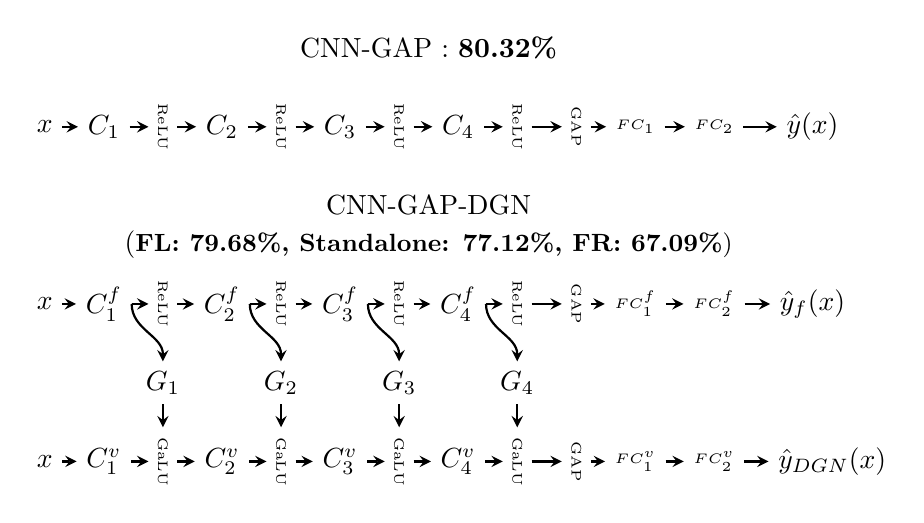
\begin{tikzpicture}
\node []  (dnn-text)at (5.375,2) {CNN-GAP : \textbf{80.32\%}};

\node []  (dnn-output) at (10.25,1) {$\hat{y}(x)$};
\node []  (dnn-fc2) at (9.0,1) {\tiny{$FC_2$}};
\draw [-stealth,thick]   (dnn-fc2.east) -- (dnn-output.west);

\node []  (dnn-fc1) at (8,1) {\tiny{$FC_1$}};
\draw [-stealth,thick]   (dnn-fc1.east) -- (dnn-fc2.west);

\node [rotate=-90]  (dnn-gap) at (7.25,1) {\tiny{GAP}};
\draw [-stealth,thick]   (dnn-gap.north) -- (dnn-fc1.west);

\node [rotate=-90] (dnn-relu-4) at (6.5,1){\tiny{ReLU}};
\node [] (dnn-c4) at (5.75,1){{$C_4$}};
\draw [-stealth,thick]   (dnn-c4.east) -- (dnn-relu-4.south);
\draw [-stealth,thick]   (dnn-relu-4.north) -- (dnn-gap.south);



\node [rotate=-90] (dnn-relu-3) at (5,1){\tiny{ReLU}};
\node [] (dnn-c3) at (4.25,1){{$C_3$}};
\draw [-stealth,thick]   (dnn-c3.east) -- (dnn-relu-3.south);
\draw [-stealth,thick]   (dnn-relu-3.north) -- (dnn-c4.west);


\node [rotate=-90] (dnn-relu-2) at (3.5,1){\tiny{ReLU}};
\node [] (dnn-c2) at (2.75,1){{$C_2$}};
\draw [-stealth,thick]   (dnn-c2.east) -- (dnn-relu-2.south);
\draw [-stealth,thick]   (dnn-relu-2.north) -- (dnn-c3.west);

\node [rotate=-90] (dnn-relu-1) at (2,1){\tiny{ReLU}};
\node [] (dnn-c1) at (1.25,1){{$C_1$}};
\draw [-stealth,thick]   (dnn-c1.east) -- (dnn-relu-1.south);
\draw [-stealth,thick]   (dnn-relu-1.north) -- (dnn-c2.west);



\node [] (dnn-input) at (0.5,1){$x$};
\draw [-stealth,thick]   (dnn-input.east) -- (dnn-c1.west);


%%%%%%%%%%%%%%%%%%%%%%%%%%%%%%%%%%%%%%%%%%%%%%%%%%%%%%%%%%%%%%%%%
\node []  (fntext)at (5.375,0) {CNN-GAP-DGN};
\node []  (fntext)at (5.375,-.5) {(\small{\textbf{FL: 79.68\%, Standalone: 77.12\%, FR: 67.09\%}})};

%\node []  (output) at (7.5,1.5) {$\hat{y}(x)$};


\node [align=right]  (dgn-f-output) at (10.25,-1.25) {$\hat{y}_{\text{f}}(x)$};
\node []  (dgn-f-fc2) at (9.0,-1.25) {\tiny{$FC^{\text{f}}_2$}};
\draw [-stealth,thick]   (dgn-f-fc2.east) -- (dgn-f-output.west);


\node []  (dgn-f-fc1) at (8,-1.25) {\tiny{$FC^{\text{f}}_1$}};
\draw [-stealth,thick]   (dgn-f-fc1.east) -- (dgn-f-fc2.west);




\node [rotate=-90]  (dgn-f-gap) at (7.25,-1.25) {\tiny{GAP}};
\draw [-stealth,thick]   (dgn-f-gap.north) -- (dgn-f-fc1.west);


\node [rotate=-90] (dgn-relu-4) at (6.5,-1.25){\tiny{ReLU}};
\node [] (dgn-f-c4) at (5.75,-1.25){{$C^{\text{f}}_4$}};
\draw [-stealth,thick]   (dgn-f-c4.east) -- (dgn-relu-4.south);
\draw [-stealth,thick]   (dgn-relu-4.north) -- (dgn-f-gap.south);


\node [rotate=-90] (dgn-relu-3) at (5,-1.25){\tiny{ReLU}};
\node [] (dgn-f-c3) at (4.25,-1.25){{$C^{\text{f}}_3$}};
\draw [-stealth,thick]   (dgn-f-c3.east) -- (dgn-relu-3.south);
\draw [-stealth,thick]   (dgn-relu-3.north) -- (dgn-f-c4.west);


\node [rotate=-90] (dgn-relu-2) at (3.5,-1.25){\tiny{ReLU}};
\node [] (dgn-f-c2) at (2.75,-1.25){{$C^{\text{f}}_2$}};
\draw [-stealth,thick]   (dgn-f-c2.east) -- (dgn-relu-2.south);
\draw [-stealth,thick]   (dgn-relu-2.north) -- (dgn-f-c3.west);


\node [rotate=-90] (dgn-relu-1) at (2,-1.25){\tiny{ReLU}};
\node [] (dgn-f-c1) at (1.25,-1.25){{$C^{\text{f}}_1$}};
\draw [-stealth,thick]   (dgn-f-c1.east) -- (dgn-relu-1.south);
\draw [-stealth,thick]   (dgn-relu-1.north) -- (dgn-f-c2.west);



\node [] (dgn-f-input) at (0.5,-1.25){$x$};
\draw [-stealth,thick]   (dgn-f-input.east) -- (dgn-f-c1.west);

\node [align=right]  (dgn-output) at (10.5,-3.25) {$\hat{y}_{\text{DGN}}(x)$};

\node [] (dgn-fc2) at (9,-3.25){\tiny{$FC^{\text{v}}_2$}};
\draw [-stealth,thick]   (dgn-fc2.east)--(dgn-output.west);

\node [] (dgn-fc1) at (8,-3.25){\tiny{$FC^{\text{v}}_1$}};
\draw [-stealth,thick]   (dgn-fc1.east)--(dgn-fc2.west);

\node [rotate=-90] (dgn-gap) at (7.25,-3.25){\tiny{GAP}};
\draw [-stealth,thick]   (dgn-gap.north)--(dgn-fc1.west);



\node [rotate=-90] (dgn-galu-4) at (6.5,-3.25){\tiny{GaLU}};
\draw [-stealth,thick]   (dgn-galu-4.north) -- (dgn-gap.south);

\node [] (dgn-v-c4) at (5.75,-3.25){{$C^{\text{v}}_4$}};
\draw [-stealth,thick]   (dgn-v-c4.east) -- (dgn-galu-4.south);

\node [rotate=-90] (dgn-galu-3) at (5,-3.25){\tiny{GaLU}};
\node [] (dgn-v-c3) at (4.25,-3.25){{$C^{\text{v}}_3$}};
\draw [-stealth,thick]   (dgn-v-c3.east) -- (dgn-galu-3.south);
\draw [-stealth,thick]   (dgn-galu-3.north) -- (dgn-v-c4.west);



\node [rotate=-90] (dgn-galu-2) at (3.5,-3.25){\tiny{GaLU}};
\node [] (dgn-v-c2) at (2.75,-3.25){{$C^{\text{v}}_2$}};
\draw [-stealth,thick]   (dgn-v-c2.east) -- (dgn-galu-2.south);
\draw [-stealth,thick]   (dgn-galu-2.north) -- (dgn-v-c3.west);


\node [rotate=-90] (dgn-galu-1) at (2,-3.25){\tiny{GaLU}};
\node [] (dgn-v-c1) at (1.25,-3.25){{$C^{\text{v}}_1$}};

\draw [-stealth,thick]   (dgn-v-c1.east) -- (dgn-galu-1.south);
\draw [-stealth,thick]   (dgn-galu-1.north) -- (dgn-v-c2.west);




\node [] (dgn-input) at (0.5,-3.25){$x$};
\draw [-stealth,thick]   (dgn-input.east) -- (dgn-v-c1.west);




\node[] (dgn-gating-1) at (2,-2.25){$G_1$};
\draw [-stealth,thick]   (dgn-f-c1.east) to[out=-90,in=90] (dgn-gating-1.north);
\draw [-stealth,thick]   (dgn-gating-1.south) -- (dgn-galu-1.west);


\node[] (dgn-gating-2) at (3.5,-2.25){$G_2$};
\draw [-stealth,thick]   (dgn-f-c2.east) to[out=-90,in=90] (dgn-gating-2.north);
\draw [-stealth,thick]   (dgn-gating-2.south) -- (dgn-galu-2.west);



\node[] (dgn-gating-3) at (5,-2.25){$G_3$};
\draw [-stealth,thick]   (dgn-f-c3.east) to[out=-90,in=90] (dgn-gating-3.north);
\draw [-stealth,thick]   (dgn-gating-3.south) -- (dgn-galu-3.west);


\node[] (dgn-gating-4) at (6.5,-2.25){$G_4$};
\draw [-stealth,thick]   (dgn-f-c4.east) to[out=-90,in=90] (dgn-gating-4.north);
\draw [-stealth,thick]   (dgn-gating-4.south) -- (dgn-galu-4.west);

	
\end{tikzpicture}


}
\end{minipage}
\end{minipage}
\caption{DGN}
\label{fig:dgn}
\end{figure}


%\cite{npk} addressed these issues by measuring the performance of the fixed gates. For this, they considered a DGN setup, wherein, the feature network is frozen so as to fix the gates and only the value network is trained. In other words, the gates are fixed the `path features' are fixed, only the `path value' is learnt in the value network. 
%As mention in \Cref{sec:intro}, the key insight in \cite{npk} is that gates play an important role in DNNs with ReLUs. The DGN has external gating, i.e., gates are generated in the feature network and are external to the value network which learns the weights. Note that the neural path features encode the input and the gates, and in the context of DGN, we will be using neural path features as a synonym for the gates. Also the neural path value is learnt in the value network, and in the context of the DGN, we will use neural path value as a synonym for weights. The following question related to learning with external gating lead to the conclusion that gates are key.

%During training, a DNN learns the relation $\hat{y}(x)=\ip{\phi_\Theta(x),v_\Theta}$, i.e., it learns both the neural path features and value. The DGN separately stores $\phi(x)$ and $v$ in the feature and value network respectively and helps in understanding their roles separately.  
%if the feature network weights are fixed, then the gates are fixed and hence the neural path features are fixed as well. 
%Now, training the value network after fixing the gates is linear in the dual variables, and we call this \textbf{dual linearity}. In other words, $\hat{y}_{\text{DGN}}(x)=\ip{\phi_{\Tf}(x),v_{\Tv}}$, is a linear model, where the neural path feature $\phi_{\Tf}(x)\in\R^{\text{total\,paths}}$ is given, and the neural path value $v_{\Tv}\in\R^{\text{total\,paths}}$ needs to be learnt. However, unlike a linear model the various coordinates of $v_{\Tv}$ are not independent variables, but are dependent on each other through the weights (see \Cref{def:npf-npv}). Thus the relation $\hat{y}_{\text{DGN}}(x)=\ip{\phi_{\Tf}(x),v_{\Tv}}$, is non-linear in the weights of the value network. This brings us to the following natural questions, which were answered using the DGN setup:


%The dual view provides the first step in disentangling the linear and the non-linear operations. To elaborate,  it is worthwhile to ask `assuming that we have the \emph{right} neural path features $\phi_{\Tf}(x)$, then can we learn $v_{\Tv}$ separately?'.  This question is worthwhile because, while in each layer of the value network GaLUs and the linear operations are entangled, disentanglement happens in the path variables, i.e., the relation $\hat{y}_{\text{DGN}}(x)=\ip{\phi_{\Tf}(x),v_{\Tv}}$ is linear in the dual variables; we call this \textbf{dual linearity}. Thus, when it comes to the value network alone, we can choose to interpret the computations in a path-by-path manner using dual linearity. This brings us to the next questions of (i) does dual linearity hold in practice?, (ii) are neural path features learnt, and (iii) how to characterise dual linearity analytically, and (iv) can the DGN be an alternative to a DNN? These questions were answered using a DGN setup based on network with $4$ convolutional layers with global average pooling as shown in \Cref{fig:dgn}. 
%\subsection{Experimental Results: Learning in the Gates}


%$\bullet$ \textbf{Fixed Learnt (FL)} gates. Here, the feature network (which is a DNN with ReLU) is \emph{pre-trained} with $\hat{y}_f$ as the output. Then the feature network is frozen and the value network is trained, i.e., in $\hat{y}_{\text{DGN}}(x)=\ip{\phi_{\Tf}(x),v_{\Tv}}$, $\phi_{\Tf}(x)$ is fixed and only $v_{\Tv}$ is learnt. Here, `hard'-gating is used: for pre-activation $q\in\R$, the gating value is $G(q) = \mathbbm{1}_{\{q>0\}}$. It was shown that \emph{most useful information is in the gates/neural path features}, i.e., using a pre-trained DNN as feature network, we can train the value network separately from scratch and match the performance of the pre-trained DNN.  See in \Cref{fig:dgn} the performance of DNN ($80.32$) is close (within $1\%$) to that of the DGN ($79.68$).

%$\bullet$ \textbf{Fixed Random (FR)} gates is similar to the FL gates, expect that, in the `FR gates' the feature network is randomly initialised and kept frozen, and only the value network is trained. Here too, hard gating is used. It was shown that  random gates/neural path features perform significantly poorly than the learnt gates/neural path features. See in \Cref{fig:dgn} the performance of DGN in the FR mode ($68.08$) which is poorer by more than $11\%$ when compared to FL mode ($79.68$).

%\textbf{Message.} Since the random gates performed poorly than the NTK and the learnt gates performed better than the NTK and close to the original DNN itself, it was concluded that (i) gates (encoded as neural path features) are learnt, and (ii) the learning in the gates is the reason for finite width DNN outperforming infinite width NTK. \cite{npk} also showed that the gates and the weights can be learnt simultaneously in a DGN. This is answered by operating the DGN in the \textbf{decoupled learning (DL)} mode, wherein, both the feature and value networks are trained starting from random initialisation. Here, `soft'-gating is used, where, $G(q)=\frac{1}{1+\exp({-\beta\cdot q})}$ ($\beta=$ 4 or 10 are typical choices): this enables gradient to flow via the feature network. It was shown that DGN performs only marginally poorly compared to a DNN. See in \Cref{fig:dgn} the performance of DGN in the DL mode ($77.12$) which is poorer by only around than $3\%$ when compared to DNN ($80.32$). 


%In other words, using pre-trained $\phi_{\Tg}(x)$ we can train the $v_{\Tv}$, in a manner analogous to linear models wherein given the features we can train the weights. 
%\textbf{Key Takeaways.} The dual view gives us an alternate way to look at feature learning. We know that $\phi(x)$s are features using which we can learn $v$s, and that $\phi(x)$s are learnt, and also that the information in the 
%\textbf{DGN Training.} The primary use of the DGN was to measure the information in the gates of a DNN with ReLU. For this, the feature network (which is a DNN with ReLU) is \emph{pre-trained} with $\hat{y}_f$ as the output. Then the feature network is frozen and the value network is trained, i.e., in $\hat{y}_{\text{DGN}}(x)=\ip{\phi_{\Tf}(x),v_{\Tv}}$, $\phi_{\Tf}(x)$ is fixed and only $v_{\Tv}$ is learnt. Here, `hard'-gating is used: for pre-activation $q\in\R$, the gating value is $G(q) = \mathbbm{1}_{\{q>0\}}$. The secondary use of DGN is as an alternative/competetive model (for DNN) that learns  $\hat{y}_{\text{DGN}}(x)=\ip{\phi_{\Tf}(x),v_{\Tv}}$, by separately learning $\Tf$ and $\Tv$ starting from randomised initialisation.Here, `soft'-gating is used, where, $G(q)=\frac{1}{1+\exp({-\beta\cdot q})}$ ($\beta=10$ is a typical choice): this enables gradient to flow via the feature network. 


\begin{comment}

We now discuss the `black box'-ness issue in DNNs and the \emph{neural tangent kernel} based interpretation of DNNs, and the insights from the dual view.


Each layer of a DNN entangles the linear computation with the non-linear activations. The commonly held view  is that such entanglement is the key to success of DNNs, in that, it allows the DNN to learn sophisticated structures in a layer-by-layer manner (we call this the primal view). However, in terms of interpretability, such entanglement has an adverse effect: only the final layer is linear and amenable to a feature/weight interpretation, and neither the feature, i.e., the penultimate layer output, nor the outputs of the intermediate hidden layers are interpretable due to the presence of non-linear activations. 

Recent works [\citep{ntk,arora2019exact,cao2019generalization}] have connected the training and generalisation of DNNs to kernel methods. An important kernel associated with a DNN is its \emph{neural tangent kernel} (NTK), which, for a pair of input examples $x,x'\in\R^{\din}$, and network weights $\Theta\in\R^{\dnet}$, is given by:
\begin{align*}
 \text{NTK}(x,x')\quad = \quad \ip{\nabla_{\Theta}\hat{y}(x), \nabla_{\Theta}\hat{y}(x')}, \quad\text{where}
\end{align*}
$\hat{y}_\Theta(\cdot)\in\R$ is the DNN output. 
It was shown that, as the width of the DNN goes to infinity, the NTK matrix converges to a limiting deterministic matrix $\text{NTK}_{\infty}$, and training an infinitely wide DNN is equivalent to a kernel method with $\text{NTK}_{\infty}$. 

While the NTK provides a kernel interpretation it has the following issues: 

(i) Finite width DNN outperforms its infinite width NTK counterpart \citep{arora2019exact}, that is, the NTK does not fully explain the success of finite width DNNs.

(ii) The NTK is a fixed matrix and hence does not capture representation learning.

(iii) The NTK does not address the issue of entanglement.

We will now discuss the fundamental insights obtained due to the dual view and the DGN setup. 

\textbf{Finite Width vs Infinite Width.} To understand this issue, \cite{npk} measured the performance of fixed gates. For this, they considered a DGN setup, wherein, the feature network is weights are fixed so as to fix the gates and only the value network is trained. In other words, since the gates are fixed, the  neural path features are fixed as well, only the neural path value is learnt in the value network. They showed that the fixed gates from a randomly initialised DNN performed poorly than the NTK and that fixed gates from a pre-trained DNN performed (i) better than the infinite width NTK and (ii) close to the pre-trained DNN itself. This shows that learning in the gates, i.e., neural path features is difference between finite and infinite width networks.

\textbf{Representation Learning.} \citep{npk} showed that in an infinite width fully connected DGN with its gates fixed, the NTK is equal (up to a scalar) to the so called \emph{neural path kernel} (NPK) (equal to the Gram matrix of the neural path features). 
A key difference between the NTK and NPK is that the following: NTK is the kernel corresponding to randomised initialisation, however NPK being the Gram matrix of neural path features is entirely dependent on the input and the gates, wherein, the gates themselves can be either learnt or random. Thus, representation learning is addressed by looking at the NPK corresponding to learnt gates.

\textbf{Entanglement.} Instead of investigating the value network layer-by-layer in which GaLUs and linear operations are entangled, the dual view opens up the option of investigating the value network path-by-path. The path-by-path dual view is more natural because, the value network is \textbf{dual linear}, i.e., it learns a linear function in the neural path features. This gives a subnetwork interpretation:  for each input, only a subset of gates are active, and correspondingly only a subnetwork of the paths are active ( $\phi(x,p)= 0$ if $p$ is inactive). Also, NPK is equal to the \emph{Hadmard} product of the input Gram matrix and a correlation matrix that measures the size of the subnetwork simultaneous active for various pairs of the input examples. In short, the disentanglement happens because the dual view projects the computations onto the path variables.

\end{comment}


\begin{comment}
\begin{definition}[Overlap of active sub-networks]\label{def:overlap} 
The total number of `active' paths for both $x$ and $x'$ that pass through input node $i$ is defined to be:\\
{\centering{\centering{$\textbf{overlap}_{\Theta}(i,x,x') = \Lambda_{\Theta}(i,x,x') \eqdef \left|\{p \colon  A_{\Theta}(x,p)= A_{\Theta}(x',p)=1\}\right|/\din$}}}
\end{definition}
%\subsection{NPK of FC-DNN: Product Kernel }
%\input{cnpkexample}
%\subsection{Neural Path Kernel : Similarity based on active sub-networks}
\begin{lemma}[Neural Path Kernel (NPK)]\label{lm:npk}
Let $D\in\R^{\din}$ be a vector of non-negative entries  and for $u,u'\in\R^{\din}$ , let $\ip{u,u'}_{D}=\sum_{i=1}^{\din}D(i)u(i)u'(i)$. Let $H_{\Theta}(x,x')\eqdef\langle\phi_{\Theta}(x),\phi_{\Theta}(x') \rangle$ be the neural path kernel (NPK). Then  
\begin{align*} 
\text{NPK}_{\Theta}(x,x')= H_{\Theta}(x,x')=\ip{x,x'}_{\Lambda_{\Theta}(\cdot,x,x')} 
\end{align*}
\end{lemma}
\textbf{Remark.} In the case of fully connected networks, $\textbf{overlap}_{\Theta}(i,x,x')$ is equal for all $i\in[\din]$, and hence $\text{NPK}_{\Theta}(x,x')=\ip{x,x'}\cdot\textbf{overlap}_{\Theta}(x,x')$.
\end{comment}
